% Finished September 26, 2013
% Put into VUW Thesis format Wednesday 2 April 2014

\documentclass[12pt, a4paper, twoside, openright]{book}

\usepackage{vuwthesis} % sets up some local things, mostly the front page

\setlength{\intextsep}{12pt} % set space above and below in-line float
\setlength{\abovecaptionskip}{0pt} % set space between figure and caption.

\usepackage{url}

\usepackage{amssymb, amsmath}
%\usepackage{mathtools}
\usepackage{tikz}
\usetikzlibrary{calc}

\newcommand{\beff}{\ensuremath{b_{\mathrm{eff}}}}
\newcommand{\bmin}{\ensuremath{b_{\mathrm{min}}}}
\newcommand{\bmax}{\ensuremath{b_{\mathrm{max}}}}
\newcommand{\bfar}{\ensuremath{b_{\mathrm{far}}}}

\newcommand{\Tr}{\ensuremath{T_{\mathrm{room}}}}

\newcommand{\Finc}{\ensuremath{F_{\mathrm{inc}}}}
\newcommand{\Fads}{\ensuremath{F_{\mathrm{ads}}}}
\newcommand{\Fdes}{\ensuremath{F_{\mathrm{des}}}}
\newcommand{\Fcat}{\ensuremath{F_{\mathrm{cat}}}}

\newcommand{\kcat}{\ensuremath{k_{\mathrm{cat}}}}
\newcommand{\kads}{\ensuremath{k_{\mathrm{ads}}}}
\newcommand{\kadscat}{\ensuremath{k_{\mathrm{ads \to cat}}}}

%\usepackage{marvosym}

\usepackage{etoolbox}
\newtoggle{compilealone}
\toggletrue{compilealone}

\title{Chapter 9: Analogues of Effective Slip}
\author{Nat Lund}

\begin{document}
\chapter{Analogues of Effective Slip}\label{C:analogs}

We have found the effective slip length for Stokes flow over a periodic mixed-slip surface.  However, on a purely mathematical level we have shown that if Laplace's equation holds on a domain, and a particular boundary condition holds on a boundary:
\begin{gather}
\nabla^2 u = f \\
u = b(x,y) \frac{\partial u}{\partial z}
\end{gather}
where $b$ is some periodic function on the boundary with units of length and period $L$,
then there exists an effective boundary parameter $\beff$ that is a good approximation in the appropriate limits:
\begin{equation}
\beff = \left< \frac{1}{b} \right>^{-1} \text{   if   } L \ll b, \qquad \text{and} \qquad
\beff = \left< b \right> \text{   if   } b \ll L
\end{equation}


%\vspace{1em}
This models our slip problem.  It is also interesting to ask what other physical systems these results might apply to.  If we can find appropriate systems, then we automatically have an effective boundary parameter --- some analogue of effective slip length.

We shall investigate two such physical systems forthwith: a thermal insulation problem and a heterogeneous catalyst problem.


\section{Thermal Insulation}

Consider an atypical New Zealand house: one with insulation in the roof.  A standard house has an angled roof situated above a flat ceiling, with a fairly large crawlspace in between.  The ceiling panels are attached to the underside of wooden beams known as rafters, which are spaced 600 mm apart.  It is traditional to devote several entire weekends to laying insulating material on top of the ceiling panels, in the gaps between the rafters.
Thus, above the warm living space of a house, is a heterogeneous insulator, comprising wood (the rafters), highly insulating material, and those air gaps that are left over because you couldn't be bothered cutting scratchy, unwieldy fibreglass batts to exactly the right size.  A schematic is presented in Figure (\ref{house}).

\begin{figure}[ht]
\centering
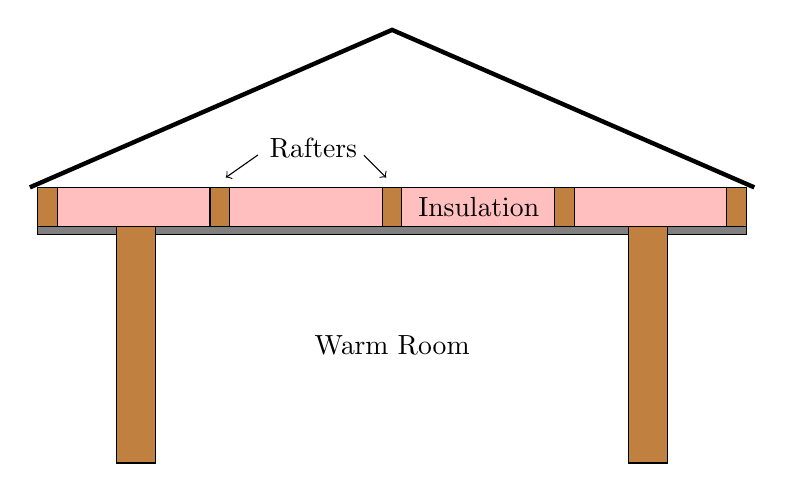
\begin{tikzpicture}
%Walls and ceiling
\draw[fill=brown] (0,0) rectangle ++(-0.5,-3);
\draw[fill=brown] (6,0) rectangle ++(0.5,-3);
\draw[fill=gray] (0,0) rectangle ++(6,-0.1);
\draw[fill=gray] (-1.5,0) rectangle ++(1,-0.1);
\draw[fill=gray] (6.5,0) rectangle ++(1,-0.1);

%Roof
\draw[fill=brown] (-1.5,0) rectangle ++(0.25,0.5);
\draw[fill=brown] (7.5,0) rectangle ++(-0.25,0.5);
\draw[ultra thick] (-1.6,0.5) -- ++(4.6,2) -- ++(4.6,-2);

% Rafters
\foreach \x in {1,2,3}
        {\draw[fill=brown] (-1.5,0) ++(\x*1.9375,0) ++(\x*0.25,0) rectangle ++(0.25,0.5);}

% Fibreglass batts
\foreach \x in {0,1,2,3}
        {\draw[fill=pink] (-1.25,0) ++(\x*1.9375,0) ++(\x*0.25,0) rectangle ++(1.9375,0.5);}

\node at (3,-1.5) {Warm Room};
\node at (2,1) {Rafters};
\draw[<-] (-1.25,0) ++(1.9375,0) ++(0.2,0.625) -- ++(35:0.5cm);
\draw[<-] (-1.25,0) ++(1.9375,0) ++(0.25,0) ++(1.9375,0) ++(0.05,0.625) -- ++(135:0.4cm);
\node at (4.1,0.25) {Insulation};

\end{tikzpicture}
\caption{Schematic of ceiling insulation in a house.}\label{house}
\end{figure}

\subsection{Mathematical Model}

We are interested in the `net' insulating properties of the heterogeneous insulator comprising wood, insulating material and possibly air gaps.  To that end, we model the heterogeneous insulator as a bulk material
with: a warm room at the lower boundary, and convection-dominated heat loss on the top boundary.  For consistency with our slip model, we shall invert the vertical dimension, and let $z=0$ denote the top of the bulk and $z=P$ the bottom of the bulk.  The temperature field is $T(x,y,z)$, with boundary conditions at $T(x,y,0)$ and $T(x,y,P)$, denoted $T(0)$ and $T(P)$.  See Figure (\ref{insulationdomain}).

\begin{figure}[ht]
\centering
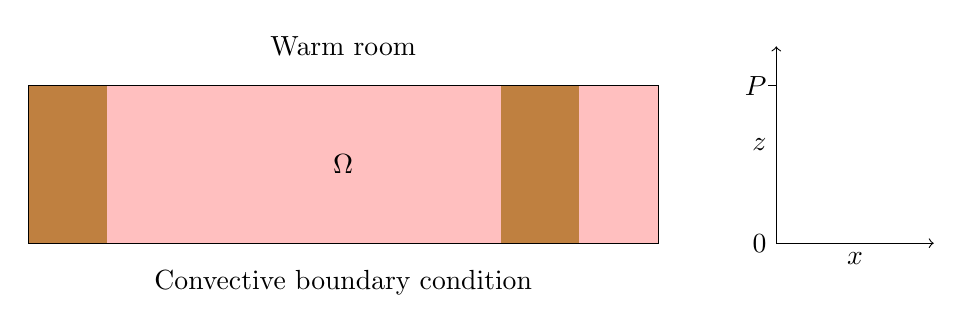
\begin{tikzpicture}

\fill[color=brown] (0,0) rectangle ++(1,2);
\fill[color=pink] (1,0) rectangle ++(5,2);
\fill[color=brown] (6,0) rectangle ++(1,2);
\fill[color=pink] (7,0) rectangle ++(1,2);

\draw (0,0) rectangle ++(8,2);

\node at (4,2.5) {Warm room};
\node at (4,1) {$\Omega$};
\node at (4,-0.5) {Convective boundary condition};

\draw[<->] (9.5,2.5) -- node[left]{$z$} ++(0,-2.5) -- node[below]{$x$} ++(2,0);
\draw (9.5,2) -- ++(-0.1,0);
\node at (9.5,2)[left]{$P$};
\node at (9.5,0)[left]{0};

\end{tikzpicture}
\caption{The domain $\Omega$ is the wooden rafters plus any insulating material.
For consistency with the slip model, the domain is `upside down'.}
\label{insulationdomain}
\end{figure}


\subsubsection{Dirichlet Condition}

The warm room can be considered to be held at a constant temperature, due to the interventions of its human occupants.  Therefore, on the $z=P$ boundary is the Dirichlet condition
\begin{equation}
T(P) = \Tr = \text{constant}
\end{equation}

\subsubsection{Bulk Condition}

The distribution of temperature $T$ in a material is governed by the heat equation:
\begin{equation}
\frac{\partial T}{\partial t} = \frac{k}{\rho C_p} \nabla^2 T
\end{equation}
where $k$ is the thermal conductivity, and $C_p$ is the specific heat capacity.

We shall assume that the system is steady-state, so that the time dependent term vanishes.  Hence, the solid material -- wooden rafters and insulating material -- is governed simply by Laplace's equation:
\begin{equation}
\nabla^2 T = 0
\end{equation}

\subsubsection{Conductive Heat Current}
Consider a bar of test material of cross-sectional area $A$ clamped between a hot reservoir and a cold reservoir, as shown in Figure (\ref{conduction}).

\begin{figure}[ht]
\centering
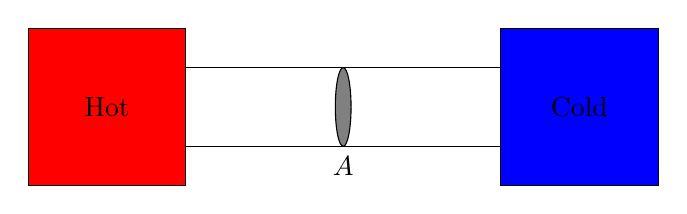
\begin{tikzpicture}
\draw[fill=red](0,-0.5) rectangle node{Hot} ++(-2,2);

\draw(0,0) rectangle ++(4,1);
\draw(0,0) ++(4,-0.5)[fill=blue] rectangle node{Cold} ++(2,2);

\draw (2,0.5)[fill=gray] ellipse (0.1cm and 0.5cm);
\node at (2,0) [below] {$A$};

\end{tikzpicture}
\caption{Bar of material of cross-section $A$ between hot and cold reservoirs.}\label{conduction}
\end{figure}

The heat current in the bar (Joules per second) depends on the temperature gradient, the thermal conductivity $k$ and the area $A$:
\begin{equation}
\frac{dQ}{dt} = k A \frac{\partial T}{\partial x}
\end{equation}


\subsubsection{Convective Heat Current}
Convection is harder to quantify than conduction.   
A plate at temperature $T$ convecting into an infinite reservoir of gas at temperature $T_0$ shows a heat flux approximately proportional to $(T - T_0)^{5/4}$.
However, consider the experimental setup in the diagram of Figure (\ref{convection}): a body of convecting air between a hot body and a cold body.


\begin{figure}[ht]
\centering
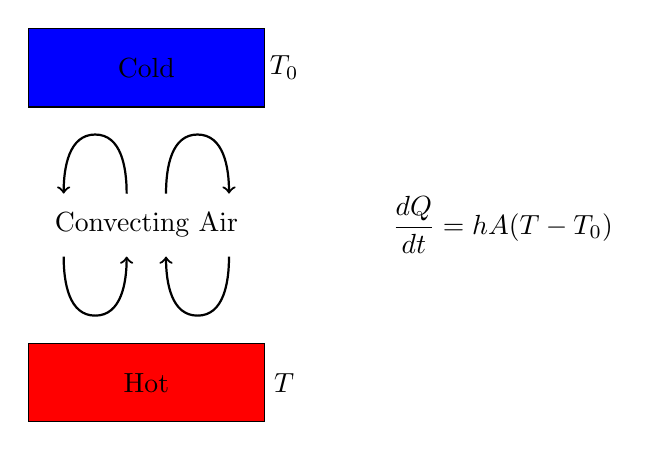
\begin{tikzpicture}
%\everymath{\displaystyle}

\node at (0,0) {Convecting Air};
\draw[fill=red] (-1.5,-1.5) rectangle node {Hot} ++(3,-1);
\draw[fill=blue] (-1.5,1.5) rectangle node {Cold} ++(3,1);

\node at (3,0)[right] {$\displaystyle \frac{dQ}{dt} = h A (T - T_0) $};

\node at (1.75,-2) {$T$};
\node at (1.75,2)  {$T_0$};

%Curved Arrows
\draw[->,thick] (0.25,0.4) to [out=90,in=180] ++(0.4,0.75) to [out=0,in=90] ++(0.4,-0.75);
\draw[->,thick] (-0.25,0.4) to [out=90,in=0] ++(-0.4,0.75) to [out=180,in=90] ++(-0.4,-0.75);
\draw[<-,thick] (0.25,-0.4) to [out=-90,in=180] ++(0.4,-0.75) to [out=0,in=-90] ++(0.4,0.75);
\draw[<-,thick] (-0.25,-0.4) to [out=-90,in=0] ++(-0.4,-0.75) to [out=180,in=-90] ++(-0.4,0.75);

\end{tikzpicture}
\caption{Convection between hot and cold reservoirs of surface area $A$.}\label{convection}
\end{figure}

For such a system, the heat flux is usually considered to have a simple linear relationship to temperature difference:
\begin{equation}
\frac{dQ}{dt} = h A (T - T_0)
\end{equation}

This is known as Newton's law of cooling. $h$ is the \emph{heat transfer coefficient} of the system, and depends on the fluid and the physical situation.

%\clearpage
\subsubsection{Convective Boundary Condition}

The highly-conductive steel roof of a house can be presumed to be at the same low temperature $T_0$ as the outside air. We assume that radiative heat transfer is negligible, and that the only heat transfer is due to convection occurring between the bulk heterogeneous insulator and the cold roof. 

The heat flux \emph{leaving} the boundary is given approximately by Newton's law of cooling.
Furthermore, heat flux will arrive \emph{at} the boundary in accordance with the heat conduction equation.  See Figure (\ref{boundaryflux}).

\begin{figure}[ht]
\centering
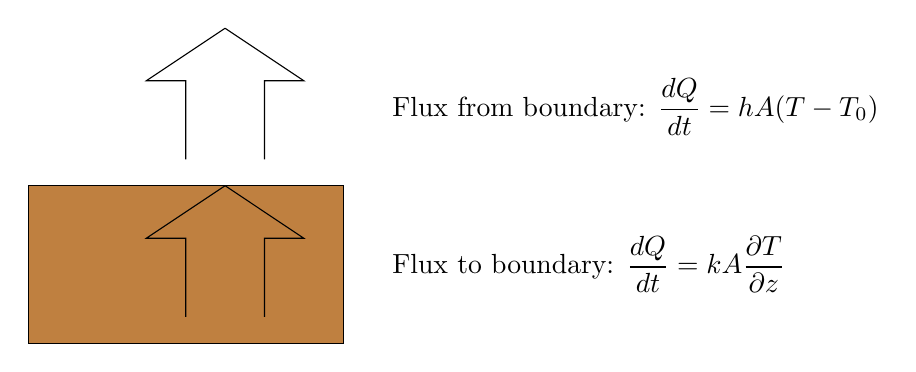
\begin{tikzpicture}
\draw[fill = brown] (1.5,0) rectangle ++(-4,-2);
\draw (0,0) -- ++(1,-0.667) -- ++(-0.5,0) -- ++(0,-1);
\draw (0,0) -- ++(-1,-0.667) -- ++(0.5,0) -- ++(0,-1);
\draw (0,2) -- ++(1,-0.667) -- ++(-0.5,0) -- ++(0,-1);
\draw (0,2) -- ++(-1,-0.667) -- ++(0.5,0) -- ++(0,-1);

\node at (2,-1)[right] {Flux to boundary: $\displaystyle \frac{dQ}{dt} = k A \frac{\partial T}{\partial z} $};
\node at (2,1) [right] {Flux from boundary: $\displaystyle \frac{dQ}{dt} = h A (T - T_0)$};

\end{tikzpicture}
\caption{Heat fluxes conducted \emph{to} boundary and convected \emph{from} boundary.}\label{boundaryflux}
\end{figure}

Since the boundary is a virtual plane with no heat capacity, the fluxes are always equal:
\begin{equation}
h A (T - T_0) = k A \frac{\partial T}{\partial z}
\end{equation}

For convenience, define a new variable $ \tau = T - T_0$.  Then the convective boundary condition is:
\begin{equation}
\tau = \frac{k}{h} \frac{\partial \tau}{\partial z}
\end{equation}

The heat transfer coefficient $h$ is constant for a given system.  But the thermal conductivity $k$ varies spatiallly because the insulation layer is heterogenous.   Define:
\begin{equation}
b(x,y) = \frac{k}{h}
\end{equation}
Then $b(x,y)$ is periodic function on the boundary and has dimensions of length.

%\clearpage
We now have a system of equations similar to those describing Stokes flow with Navier slip:
\begin{gather}
\nabla^2 \tau = 0 \\
\tau = b \frac{\partial \tau}{\partial z}
\end{gather}

Note that while the boundary condition is heterogeneous -- $b(x,y)$ is a function of position on the boundary plane -- this is due to the fact that \emph{bulk} is heterogeneous.  The coupling occurs because the heat fluxes match at the boundary.

The function $b(x,y)$ has units of length, and we can now solve to find an effective `insulation length' for the heterogeneous insulation.
We assume that all heat in the room is ultimately lost by convection above the insulator.  Since the convective heat flux depends on the temperature on the convective boundary,
  to minimize heat loss for a given room temperature, we want the lowest temperature on the convective boundary.  This in turn demands the lowest effective insulation length.  See Figure (\ref{insulationlength}).

\clearpage

\begin{figure}[ht]
\centering
\begin{tikzpicture}
\draw [<->] (0,4) -- (0,0) -- (9,0);
\draw (4,0) -- ++(0,4);
\draw[thick, color=red] (0,3) -- (4,1.5);
\draw[thick, color=red,dashed] (4,1.5) -- (8,0);

\node at (4,0)[below] {0};
%\node at (0,0)[below] {$d$};

\draw (0,3) -- ++(-0.1,0);
\node at (-0.1,3)[left] {\Tr};

\draw[<->] (4,-0.7) -- node[below]{\beff} ++(4,0);

\draw[<->] (3.7,0) -- node[left] {$T(0)$} ++(0,1.5);

\end{tikzpicture}
\caption{Minimizing heat loss requires minimal $T(0)$, which implies minimal `insulation length' $\beff$.}\label{insulationlength}
\end{figure}


\subsection{Ready-Made Solution}

To apply one of the two formulae we have already found, we need to know which regime the system is in.  We first use empirical data on typical insulating materials to estimate a range for $b$. 

%The heterogeneity of the bulk material is due to the wooden rafters, spaced about half a meter apart.  Thus the period $L \simeq 1$m.  Rafters are 10 cm tall, so together with the ceiling material, the bulk has a height $P$ of 0.12 meters.  Therefore, the system is \emph{not} in the regime $L \ll P$, so the harmonic mean formula does not apply.

%Is the system in the regime $b \ll P$?  To find out, we first calculate $b$.

The heat transfer coefficient for air is experimentally determined to be in the range 10 - 100 Wm$^{-2}$K$^{-1}$.
The thermal conductivity for wood depends on the moisture content: from 0.04 - 0-.12 Wm$^{-1}$K$^{-1}$ for oven-dry wood, and up to 0.4 Wm$^{-1}$K$^{-1}$ for wood with more than 12\% water content.
Typical highly-insulating materials might be polystyrene foam or polyurethane foam, with $k$ = 0.03 Wm$^{-1}$K$^{-1}$, or mineral wool, sheep's wool, or fibreglass wool, at $k$ = 0.04 Wm$^{-1}$K$^{-1}$.
Air itself -- if sufficiently constrained to avoid convection -- has a very low thermal conductivity of $k$ = 0.024 Wm$^{-1}$K$^{-1}$.

Thus values of $b = k/h$ are in the range 0.0003 to 0.012 meters, i.e. at most about one centimeter.
%Clearly, $b \ll L$ so we are in the regime where the effective insulation length is given by the area-weighted average:
%Since $P$ is 0.12 meters, $b$ is at most 10\% of $P$, and thus the effective insulation length $\beff$ may be well approximated by the area-weighted average: 

This analysis of effective insulation parameter was motivated by the familiar example of ceiling insulation in a house, with domain height $P$ being the 10 - 15 centimeter thickness of ceiling insulation, and period $L$ being the rafter-to-rafter spacing of 60 centimeters.  Then $b$ is clearly much less than the other length scales.  However, in this example, we do not have $L \ll P$, so strictly speaking, none of our results can be assumed to be good approximations.  But, for general macroscale insulation layers made up of materials like those mentioned above, if they are constructed such that $L \ll P$, then we would be in the regime $b \ll L \ll P$, and the effective insulation length would be reasonably approximated by the area-weighted average:
\begin{equation}
\beff = \left< b \right>
\label{eq:effins}
\end{equation}

For `deep' insulation layers with $L \ll P$, Equation (\ref{eq:effins}) has serious implications. An insulator may be constructed with steel components, which has a thermal conductivity of around 40 Wm$^{-1}$K$^{-1}$. An air gap in the insulator may form a closed convective cell with a heat transfer coefficient of 10 - 100 Wm$^{-2}$K$^{-1}$; for convenience say 40 Wm$^{-2}$K$^{-1}$.  Then a one meter tall convection cell would have the same heat current per unit area as solid steel.  Thus, it is possible to have regions with a thermal conductivity 3 or more orders of magnitude higher than the best regions. If the worst regions occupy 1\% of the surface area, the effective insulating length is 10 times worse than if the insulator were constructed purely of a good insulator like polystyrene.
For a deep insulating layer, then, it is critical to eliminate any air gaps that are big enough to allow convection.

\vspace{1em}
An interesting historical note: The first expression for effective slip is the one by J.R. Philip from 1972.  His method `generalizes a device of Karush and Young'.  The 1952 paper by Karush and Young
dealt with the effect of a periodic array of perfectly insulating stripes or circles, that partially block the loss of heat from a lump of radioactive material.

\clearpage
\section{Catalysis}

One particularly widespread application of catalysts is in the catalytic converters fitted to the exhaust systems of motorcars.  Efforts are underway to improve these catalysts by the use of nanostructured material.  The improvement is partly from the increased surface area, and partly from a geometric effect: the sharp corners of a catalyst nanoparticle seem to be more active than flat surfaces of the same catalyst.

Thus, it is possible that a nanostructured catalyst has a catalytic activity that varies across a nominal surface  -- the catalyst is heterogeneous, and may be a candidate for modelling as a homogenization problem.  We shall attempt this here.

\vspace*{1em}
Figure (\ref{catalyst}) is a schematic diagram of a catalyst in action.  We shall consider the simplest case of a single gas species -- say N$_2$O$_4$, that diffuses to the surface of the catalyst, where a catalysed reaction breaks the molecule down into separate N$_2$ and O$_2$ molecules.  The catalyst surface has some `sharp bits' that have greater catalytic activity than the flat regions.



\begin{figure}[ht]
\centering
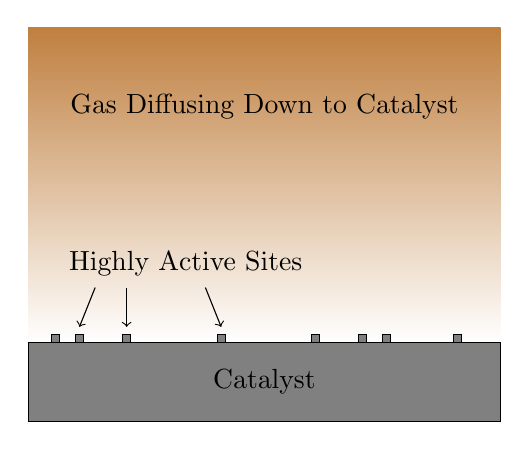
\begin{tikzpicture}

\shade[top color=brown] (0,0) rectangle ++(6,4);
\draw[fill=gray] (0,0) rectangle node {Catalyst} ++(6,-1);

\foreach \x in {0.5,1,2, 4, 6,7,7.5, 9}
                      {
                      \draw[fill=gray]  (6* \x/10, 0) rectangle ++(0.1,0.1);
                      }
 
\node at (2,1) {Highly Active Sites};
\draw[<-] (0.65,0.2) -- ++(0.2,0.5);
\draw[<-] (1.25,0.2) -- ++(0.0,0.5);
\draw[<-] (2.45,0.2) -- ++(-0.2,0.5);

\node at (3,3) {Gas Diffusing Down to Catalyst};


\end{tikzpicture}
\caption{Schematic of a catalyst with surface structure.}\label{catalyst}
\end{figure}

\subsection{Model}

The concentration of the gas species (eg. N$_2$O$_4$) is $C$.  The presence of the reaction products is presumed to not influence the behaviour of the gas species, so they are ignored.
\vspace*{1em}

The system is a flat (ish) plane of catalytic material, with gas flowing past parallel to the surface.  The velocity of the gas is not important; the gas species of interest \emph{diffuse} down to the surface.  At some height $P$ above the surface, the gas concentration can be considered static, constantly being replenished by uncatalysed exhaust gas.  Thus the system is `driven' by a fixed concentration $C_P$ at the top of the domain.  The size of $P$ depends on how the catalyst is engineered; for example the catalyst could consist of hundreds of parallel pipes, each with a diameter of several millimeters.  Then $P$ would be the radius of a pipe, with a magnitude of several millimeters.

%The system is `driven' by a fixed concentration of gas in the exhaust gases flowing past.  This gives the top boundary condition as $C(top) = C_D$.


\subsubsection{Bulk Condition: Laplace}

Oxides of nitrogen comprise less than 1\% of exhaust gas, so our gas species is very dilute, and so its concentration is governed by the diffusion equation.  Furthermore, we shall assume steady-state conditions, so the time-dependent term vanishes, and the bulk gas obeys Laplace's equation:
\begin{equation}
\nabla^2 C = 0
\end{equation}


\subsubsection{Boundary Layer}

For convenience, we shall define the layer of gas adjacent to the surface as the \textbf{boundary layer.}  All atoms that rain down onto the surface come from the boundary layer. There are four fluxes of molecules associated with the boundary layer: the flux of particles \emph{into} the boundary layer from the bulk gas; the flux of particles that adsorb to the surface; the flux of particles that desorb from the surface before being catalysed; and the virtual flux of molecules destroyed by the catalyst, that leave the boundary layer by ceasing to exist. These fluxes are illustrated in the schematic of Figure (\ref{catalystfluxes}).

\begin{figure}[ht]
\centering
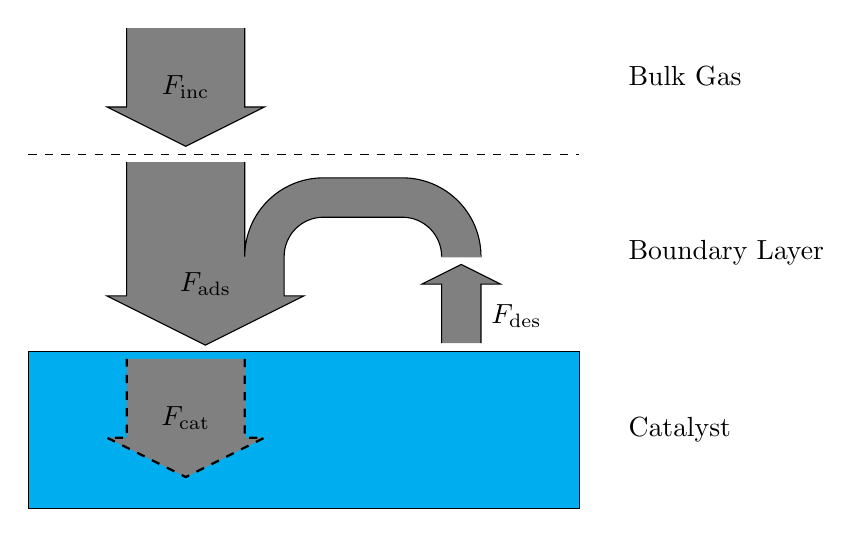
\begin{tikzpicture}
\draw[fill=cyan] (0,0) rectangle (7,-2);
\draw[dashed] (0,2.5) -- ++(7,0);

\node at (7.5,3.5)[right] {Bulk Gas};
\node at (7.5,1.25)[right] {Boundary Layer};
\node at (7.5,-1)[right] {Catalyst};

\coordinate (finc) at (2,2.6);
\draw[fill=gray] (finc) ++(0.75,1.5) -- ++(0,-1) -- ++(0.25,0) -- (finc) -- ++(-1,0.5) -- ++(0.25,0) -- ++(0,1);

\coordinate (fcat) at (2,-1.6);
\draw[thick,dashed, fill=gray] (fcat) ++(0.75,1.5) -- ++(0,-1) -- ++(0.25,0) -- (fcat) -- ++(-1,0.5) -- ++(0.25,0) -- ++(0,1);

\coordinate (fads) at (1.25,2.4);
\draw[fill=gray] (fads) -- ++(0,-1.7) -- ++(-0.25,0) -- ++(1.25,-0.625) -- ++(1.25,0.625)
-- ++(-0.25,0) -- ++(0,0.5) to [out=90,in=180] ++(0.5,0.5) -- ++(1,0)
to [out=0,in=90] ++(0.5,-0.5) -- ++(0.5,0) to [out=90,in=0] ++(-1,1) -- ++(-1,0)
to [out=180,in=90] ++(-1,-1) -- ++(0,1.2);

\draw[color=gray,fill=gray] (fads) ++(4,-1.2) -- ++(0.5,0) -- ++(-0.25,0.25);

\coordinate (fdes) at (5.25,0.1);
\draw[fill=gray] (fdes) -- ++(0,0.75) -- ++(-0.25,0) -- ++(0.5,0.25) -- ++(0.5,-0.25) -- ++(-0.25,0) -- ++(0,-0.75);


\node at (2,3.35) {\Finc};
\node at (2,-0.85) {\Fcat};
\node at (2.25,0.85) {\Fads};
\node at (6.2,0.45) {\Fdes};

\end{tikzpicture}
\caption{Balance of gas fluxes.  In the steady-state, the net molecular flux into the boundary layer must equal the (virtual) flux of catalysed molecules leaving the boundary layer.}\label{catalystfluxes}
\end{figure}


\subsubsection{Mass Balance}
There is a \emph{net} flux $\Finc$ of molecules per second entering the boundary layer.  There is a flux $\Fcat$ of molecules per second permanently leaving the boundary layer by adsorbing to the surface and being catalysed out of existence.  Eg. if we are concerned with the concentration $C$ of N$_2$O$_4$, the catalysed reaction N$_2$O$_4$ $ \to$ 2O$_2$ + N$_2$ causes the N$_2$O$_4$ molecule to cease to exist (the N$_2$ and O$_2$ detach from the catalyst and diffuse away from the surface).

In the steady state, the concentration $C$ in the boundary layer is constant, so by conservation of mass, the incoming flux must equal the outgoing flux:
\begin{equation}
\Finc = \Fcat
\end{equation}

As an aside, there may also be an auxiliary flux cycle:
In order to be catalysed, a molecule must first adsorb to the catalyst.  However, in principle, an adsorbed molecule may \emph{desorb} before being catalysed.  Thus:
\begin{equation}
\Fads = \Fcat + \Fdes
\end{equation}
A desorbed molecule may adsorb again, or it may diffuse out of the boundary layer.  Since $\Finc$ is defined as a \emph{net} incoming flux,
we may not need to worry about this.  In any case, for the sake of simplicity, we shall assume that desorption can be neglected.
% we don't need to worry about this.  Our only concern is the flux of molecules that are adsorbed and subsequently catalysed.

\subsubsection{Incoming Flux}

The flux of molecules entering the boundary layer -- moles per second per square meter -- is given by Fick's first law of diffusion:
\begin{equation}
\Finc = D \frac{\partial C}{\partial z}
\end{equation}
For an ideal gas, the diffusion coefficient $D$ is given by $\frac{1}{3} \lambda \bar{u}$, where $\lambda$ is the mean free path in the gas and $\bar{u}$ is the mean speed of gas particles.  We will use this as an approximation to the diffusion coefficient of our gas. So:
\begin{equation}
\Finc = \frac{1}{3} \lambda \bar{u} \frac{\partial C}{\partial z}
\end{equation}


\subsubsection{Catalyzed Flux}

One can imagine how the behaviour of a catalyst could be studied experimentally.
Keeping a well-mixed body of gas in contact with a catalyst at a constant temperature and pressure, for a given concentration of gas, the experimentalist will observe a certain number of moles catalysed per second (per square meter).  If the concentration is not too high, then we would expect the catalyzed flux to be proportional to concentration. That is, if we double the concentration, we double the number of molecules hitting the surface, thus double the number of opportunities for a molecule to be catalysed.  (At higher concentrations, the catalyst will saturate.)
\begin{equation}
\Fcat \propto C 
\end{equation}
We are assuming that if a molecule strikes the surface, it has an opportunity to be catalysed, and the \emph{probability} that it \emph{is} catalysed does not change with $C$.  Define $\kcat$ as the probability that a particle striking the surface is subsequently catalysed (rather than bouncing off or desorbing before being catalysed).

(It is possible to break $\kcat$ down into a probability $\kads$ that an incident particle adsorbs, and a conditional probability (per unit time) $\kadscat$ that an already-adsorbed particle is catalysed. Essentially, we are assuming that $\kadscat$ is large enough that the dwell time $1/ \kadscat$ is shorter than the mean time between impacts at a catalyst site. In the fuller treatment, one accounts for a pool of adsorbed particles that may build up if $\kadscat$ is low.
At some level of coverage, there is a non-negligible chance that an incident particle will bounce off an adsorbed particle, rather than striking the catalyst.  In these saturated conditions, $\kcat$ stops being a constant and becomes a function of $C$.
This treatment leads to the Langmuir equation.  However, the simplified treatment we give here is compatible with our effective boundary parameter expressions.)

We can apply some gas kinetics.  In Appendix A, we show that the flux incident on a surface in a gas of concentration $C$ is:
\begin{equation}
F = \frac{1}{4} \bar{u} C
\end{equation}
Since $\kcat$ is the probability that an incident particle is subsequently catalysed, the flux of particles hitting the surface and being catalysed out of existence is:
\begin{equation}
\Fcat = \frac{1}{4} \kcat \bar{u} C
\end{equation}

%(If the concentration is very high, and the `dwell time' between adsorbing and vanishing is too long, then a pool of reactants will build up on the surface.  At some level of coverage, there is a non-negligible chance that an incident particle will bounce off an adsorbed particle, rather than striking the catalyst.  In these saturated conditions, the linear relationship will break down; put another way, $\kcat$ stops being a constant and becomes a function of $C$.)


\subsubsection{Catalyst Boundary Condition}

As noted, in the steady-state, by mass balance, $\Finc = \Fcat$. Therefore:
\begin{equation}
\frac{1}{3} \lambda \bar{u} \frac{\partial C}{\partial z} = \frac{1}{4} \kcat \bar{u} C
\end{equation}
Let us introduce the catalytic parameter:
\begin{equation}
b = \frac{4}{3} \frac{\lambda}{\kcat}
\end{equation}
Then the catalyst boundary condition is:
\begin{equation}
C = b \frac{\partial C}{\partial z}
\end{equation}
which once again resembles the Navier slip condition.
Furthermore, $b$ again has units of length, since it is a multiple of the mean free path.

If the catalyst is heterogeneous, perhaps due to nanostructure, then the catalytic parameter $b(x,y)$ is a function on the surface of the catalyst.



\subsection{Solution}
We can provide a ready-made solution to
\begin{gather}
\nabla^2 C = 0 \qquad \text{in the bulk} \\
C = b \frac{\partial C}{\partial z} \qquad \text{on the boundary}
\end{gather}
provided that we know $b(x,y)$ as a function of position on the catalyst surface.
% Whether or not that is feasible is a question for chemistry, and is beyond the scope of this thesis.  This naive, physicist's analysis suggest that if it is feasible, then
The homogenization technique may be applied, and an effective parameter for catalytic activity $\beff$ can be calculated.

\vspace*{1em}
%\clearpage
Since $\kcat$ is a probability between 0 and 1, $b$ is in the range $\frac{4}{3}\lambda$ to $\infty$. The mean free path of air at standard temperature and pressure is $\lambda = 68$nm.  However temperatures and pressures in automotive catalytic converters are much higher: they need a temperature of at least 250$^{\circ}$C to work properly, and actual operating temperatures vary from 300$^{\circ}$C at idle up to 1000$^{\circ}$C if driven by bogans. Now,
\begin{equation}
\lambda = \frac{k_{\mathrm{B}} T}{\sqrt{2} \pi d^2 p}
\end{equation}
(where $k_{\mathrm{B}}$ is Boltzmann's constant, $T$ is temperature, $p$ is pressure and $d$ is the diameter of the gas particle).
So, if typical $T$ is double or triple room temperature, and $p$ is somewhat higher than ambient, then we would expect $\lambda \sim 100$nm, and similarly:
\begin{equation}
b \geq 100 \;\text{nanometers}
\end{equation}

The height of the domain $P$ depends on how the catalytic converter is engineered, but is at least millimeters.  If the catalyst is truly `nanostructured', with a period $L$ of at most tens of nanometers, then obviously $L \ll P$, and the harmonic mean formula for rough surfaces should give a good approximation for the effective catalytic parameter of the surface.  If the catalyst surface is described by the periodic function $h(x,y)$, then we have:
\begin{equation}
\beff = \left< \frac{ \sqrt{1+|\nabla h|^2} }{b} \right>^{-1}
\end{equation}

%\vspace*{1em}
Conversely, if the effective catalytic activity of a nanostuctured catalyst is measured, and compared with the standard flat plane morphology, then the activity of the most active regions of the catalyst may be estimated using the homogenized harmonic mean (or mean) formula.

\vspace*{1em}
In the dilute limit, the mean free path $\lambda$ is approximately constant.  Therefore, since $ b = \frac{4}{3} \frac{\lambda}{\kcat} $, we have
\begin{equation}
\beff = \frac{4 \lambda}{ 3 \left< \kcat \sqrt{1+|\nabla h|^2} \right> }
\end{equation}
Solving $ b = \frac{4}{3} \frac{\lambda}{\kcat} $ for $\kcat$ we may define an effective catalytic activity:
\begin{equation}
k_{\mathrm{cat (eff)}} = \frac{4 \lambda}{3 \beff}
\end{equation}
which gives:
\begin{equation}
k_{\mathrm{cat (eff)}} = \left< \kcat \sqrt{1+|\nabla h|^2} \right>
\end{equation}

Therefore, the effective catalytic activity of a nanostructured catalyst with a short dwell time and negligible desorption, is simply the average activity of its various regions, weighted by the area of contact between solid and gas.

\iftoggle{compilealone}
    {
    \bibliography{Lund_Thesis.bib}
    \bibliographystyle{plain}
    }

\end{document}


The appropriate solution regime depends on $L$ and $\kcat$.  If a `nanostructured' catalyst truly has a roughness with a period of at most tens of nanometers, then certainly $L \ll b$, regardless of $\kcat$, so that:
\begin{equation}
\beff = \left< \frac{1}{b} \right>^{-1} \quad \text{if} \quad L < \sim 100 \mathrm{nm}
\end{equation}

If on the other hand, the surface structure has a period of a micron or more, and the catalyst is reasonably efficient -- $\kcat > \sim 0.5$ -- then $b \ll L$ and:
\begin{equation}
\beff = \left< b \right> \quad \text{if} \quad L > \sim 1 \mu \mathrm{m} \;\;\; \text{and} \;\;\; \kcat > \sim 0.5
\end{equation}

If the catalyst is very inefficient, $\kcat < 0.1$, then $b$ is very sensitive to small changes in $\kcat$.  Therefore we cannot give any definite guidelines about whether the system is in the $b \ll L$ regime or the $L\ll b$ regime.
